\documentclass{article}

\usepackage{shyne}

% document format
\topmargin 0in
\oddsidemargin 0in
\evensidemargin 0in
\headheight 0in
\headsep 0in
\topskip 0in
\textheight 9in
\textwidth 6.5in
\linespread{1.3}

\begin{document}

\begin{flushleft}
\section*{Group Work - Chapter 3}
\paragraph{1} The file ``max\_temp\_dec17.csv" on D2L contains the daily high temperatures (in F) for December. 
\begin{itemize}
\item [(a)] Find the mean, median, mode and midrange of the sample. What is the most appropriate measure of center for this data?\\

\bigskip
{\centering
\begin{tabular}{cccc}
Mean & Median & Mode & Midrange \\ 
  \hline
24.65 &  25 & 22, 24, 29 & 24.50 \\ 
\end{tabular}
\par}
\bigskip
\bt{Since temperatures are roughly normal and symmetric, mean is the most appropriate measure of center.}
\vspace{.5in}
\item[(b)] Find the range, variance and standard deviation of the sample. Be sure to include the correct units for each measure.\\

\bigskip
{\centering
\begin{tabular}{ccc}
 Range & Variance & SD \\ 
  \hline
 65 \textdegree F & 252.90 (\textdegree F)$^2$ & 15.90 \textdegree F \\ 
\end{tabular}
\par}

\vspace{.5in}
\item[(c)] Within the data set, what percentile is 45 degrees? What temperature is the 10th percentile?\\

\bigskip
\bt{46 \textdegree F is the 88th percentile.\\
The 10th percentile is 3 \textdegree F.}
\end{itemize}



\newpage
\paragraph{2} The file ``mpls\_home\_sales.csv" on D2L contains the adjusted sale prices (in dollars) of a sample of home sold in Minneapolis in 2016. 
\begin{itemize}
\item [(a)] Find the mean, median, mode and midrange of the sample. What is the most appropriate measure of center for this data?\\

\bigskip
{\centering
\begin{tabular}{cccc}
Mean & Median & Mode & Midrange \\ 
  \hline
234980.59 & 202750.00 & None & 451000.00 \\ 
\end{tabular}
\par}
\bigskip
\bt{By looking at the histogram, we can see that the data is right skewed with a few extremely high values. Thus, median is the most appropriate measure of center.}

\bigskip
{\centering
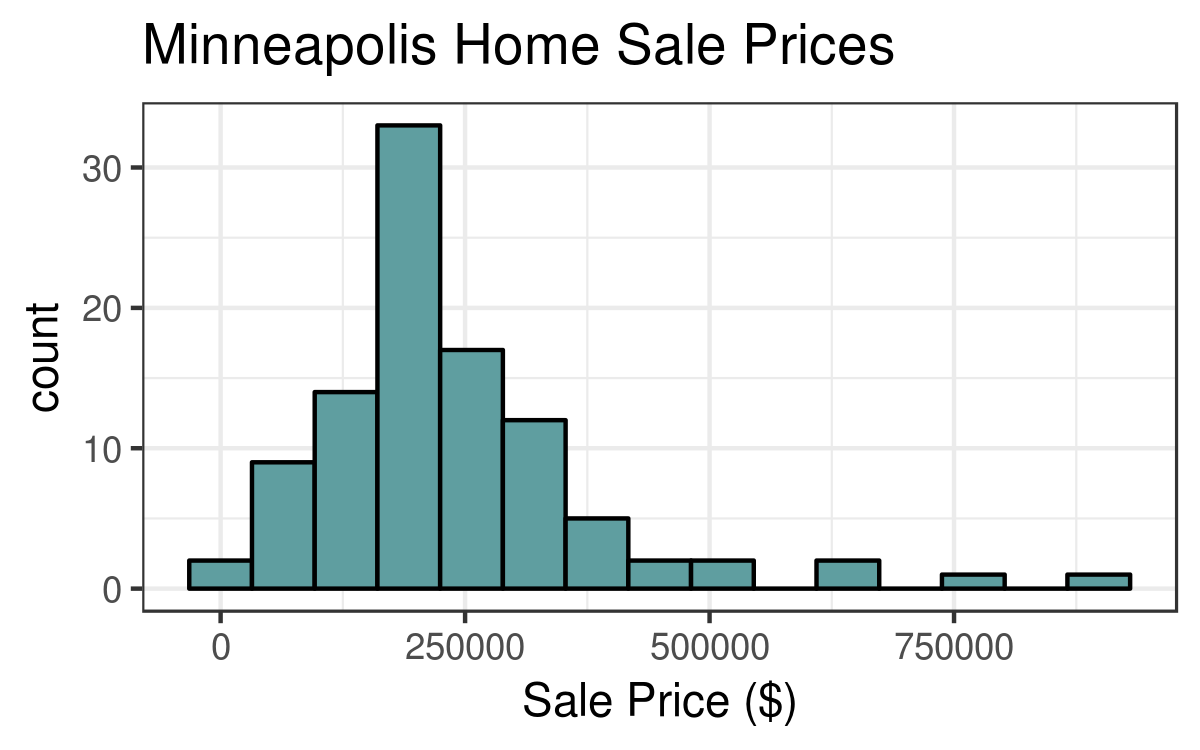
\includegraphics[width=4in]{images/grp03_Q2_a}
\par}

\vspace{.5in}
\item[(b)] Find the range, variance and standard deviation of the sample. Be sure to include the correct units for each measure.\\

\bigskip
{\centering
\begin{tabular}{ccc}
Range & Variance & SD \\ 
  \hline
898000 \$ & 21434941764.24 \$$^2$ & 146406.77 \$ \\ 
\end{tabular}
\par}
\vspace{.5in}

\newpage
\item[(c)] Find the 5 number summary of the sample and create a boxplot. What does the boxplot tell you about the distribution of the data.\\

\bigskip
{\centering
\begin{tabular}{ccccc}
Min & Q1 & Med & Q3 & Max \\ 
  \hline
2000.00 & 161250.00 & 202750.00 & 286225.00 & 900000.00 \\ 
\end{tabular}
\par}

\bigskip
{\centering
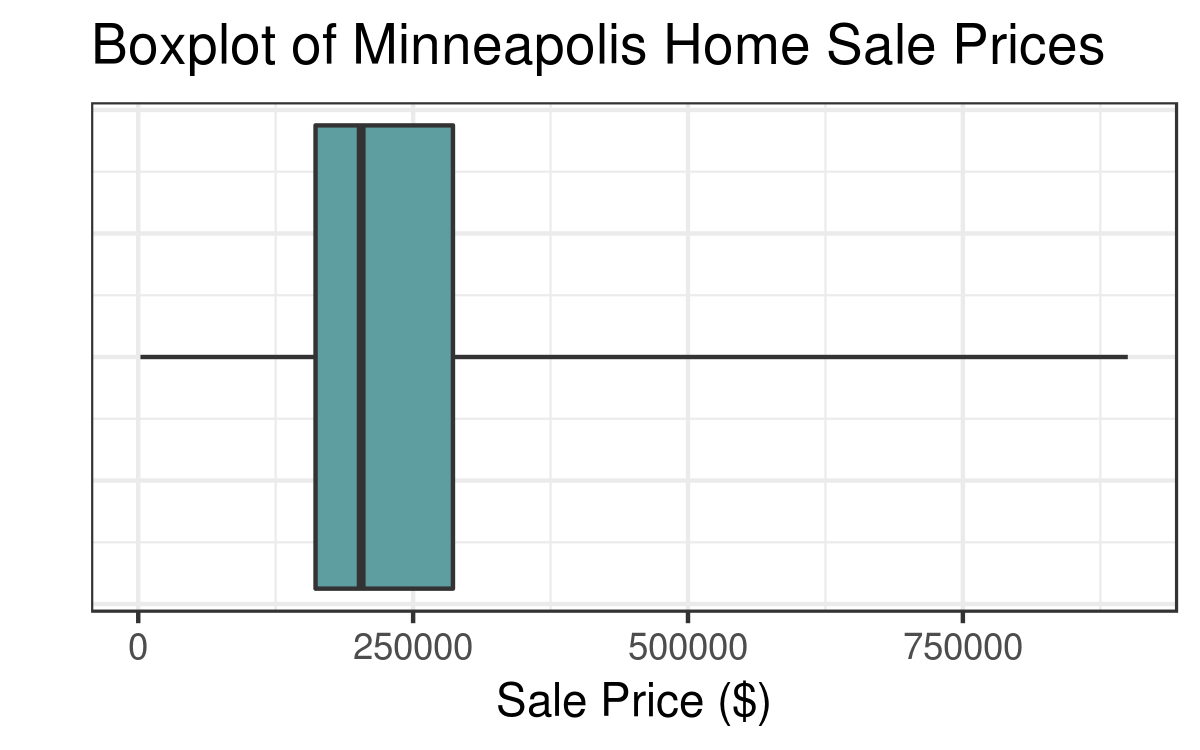
\includegraphics[width=4in]{images/grp03_Q2_c}
\par}

\bigskip
\bt{Like the histogram, the boxplot shows a heavily right skewed distribution.}
\end{itemize}

\newpage
\paragraph{3} The file ``heights.csv" on D2L contains simulated heights (in inches) of 25 men and 25 women in a statistics class. 
\begin{itemize}
\item [(a)] Find the mean and median of both samples. What is the most appropriate measure of center for this data?\\

\bigskip
{\centering
\begin{tabular}{ccc}
 & Mean & Median \\ 
  \hline
men & 70.24 & 70.30 \\ 
  women & 63.29 & 63.70 \\ 
\end{tabular}
\par}

\bigskip
\bt{We expect heights to be approximately normal, so mean is the most appropriate measure of center.}
\vspace{.5in}

\item[(b)] Find standard deviation of both samples.\\

\bigskip
{\centering
\begin{tabular}{cc}
 & SD \\ 
  \hline
men & 5.04 in \\ 
  women & 5.28 in \\ 
\end{tabular}
\par}
\vspace{.5in}


\item[(c)] Suppose two new students join the class. One is a woman who is 71 inches tall and one is a man who is 74 inches tall. Calculate z-scores for both. Who is taller for their gender? Are either of them unusually tall?\\

\bigskip

$\bv{\ds z = \frac{x - \bar x}{s}}$\\
\medskip
$\ds \bv{ z_w = \frac {71-63.29}{5.28} = 1.46 }$\\
\medskip
$\ds \bv{ z_m = \frac {74 - 70.24}{5.04} = 0.75}$\\
\bigskip
\bt{The woman has a higher z-score, so she is taller for her gender than the man is. Neither z-score is greater than 2, so neither new student has an unusual height.}
\end{itemize}


\end{flushleft}
\end{document}